\documentclass{beamer}
\usepackage[utf8]{inputenc}
\usepackage[english,russian]{babel}
\usepackage{indentfirst}
\usepackage{graphicx}
\usepackage{tikz}
\usepackage{amsmath}
\usepackage{parskip}
\usepackage[most]{tcolorbox}
\usepackage{hyperref}

\hypersetup{
	colorlinks,
	citecolor=black,
	filecolor=black,
	linkcolor=blue,
	urlcolor=blue
}

\graphicspath{{pic/}, {~/Pictures/TeXImgs/}, {../tex/pic/}}

\newcommand{\sfrac}[2]{\dfrac{\strut #1}{\strut #2}}

\newcounter{picture}
\setcounter{picture}{1}
\newcounter{tbl}
\setcounter{tbl}{1}
\newcommand{\embed}[3]{\begin{center}
		\includegraphics[scale=#2]{#1}
		\\\textbf{Рис. \thepicture:} #3
		\label{pic_\thepicture}
		\addtocounter{picture}{1}
\end{center}}
\newcommand{\embedeps}[3]{\begin{center}
		\includegraphics[width=#2\linewidth]{#1}
		\\\textbf{Рис. \thepicture:} #3
		\label{pic_\thepicture}
		\addtocounter{picture}{1}
\end{center}}
\newcommand{\embedtbl}[3]{\begin{center}
		\begin{tabular}{#1}
			#2
		\end{tabular}
		\\\textbf{Табл. \thetbl:} #3
		\label{tbl_\thetbl}
		\addtocounter{tbl}{1}
\end{center}}
\newcommand{\picref}[1]{\hyperref[pic_#1]{Рис. #1}}
\newcommand{\tblref}[1]{\hyperref[tbl_#1]{Табл. #1}}

\begin{document}
	\fontfamily{cmr}\selectfont
	\begin{frame}
		\vspace*{\fill}
		
		\begin{center}
			
\includegraphics[scale=0.3]{MIPT.png}
			\\[0.2cm] Московский Физико-Технический Институт\\(национальный исследовательский университет)
			\\[0.5cm]{\Large Отчет по эксперименту}
			\\[0.2cm]\noindent\rule{\textwidth}{1pt}
			\\\textbf{Эффект Поккельса}
			\\[-0.2cm]\noindent\rule{\textwidth}{1pt}
		\end{center}
		
		\begin{flushleft}
			\textit{Работа №4.7.2; дата: 11.03.23}\hfill\textit{Семестр: 4}
		\end{flushleft}
		
		\vspace*{\fill}
		
		\begin{flushleft}
			Выполнил: \hspace{\fill} Группа:
			\\Кошелев Александр \hspace{\fill} Б05-105
		\end{flushleft}
	\end{frame}

	\begin{frame}
		{\large \textbf{Введение:}}
		
		\textbf{Цель работы:}
		
			Исследовать интерференцию рассеянного света, прошедшего кристалл; наблюдать изменение характера поляризации света при наложении на кристалл электрического поля.
		
		\textbf{План работы:}
		
		\begin{itemize}
			\item Исследовать интерференцию на кристалле
			\item Определить двулучепреломление
			\item Определить полуволновое напряжение
			\item Проверить полуволновое изображение с помощью фигур Лиссажу
		\end{itemize}
	\end{frame}

	\begin{frame}
		{\large \textbf{Теоретическая справка:}}
		
		\textbf{Одноосный кристалл:}
		
		Одноосным называется кристалл, оптические свойства которого обладают симметрией вращения относительно некоторого направления, называемого \textit{оптической осью}.
		
		Пусть $\mathrm{o}Z$ -- оптическая ось, тогда выделяют \textit{ординарные} волны $\vec{E} \perp (\vec{k}, \vec{e_z})$ и \textit{экстраординарные} $\vec{E} \in (\vec{k}, \vec{e_z})$.
		
		Пустим волну под малым углом $\theta$ к оптической оси, тогда для ординарной волны показатель преломления $n_1 = n_o$, а для экстраординарной $n_2 = n_o- (n_o - n_e)\theta^2$, где $n_o$ -- показатель преломления вдоль оптической оси, а $n_e$ -- перпендикулярно ей.
	\end{frame}

	\begin{frame}
		\textbf{Эффект Поккельса:}
		
		\begin{figure}[h]
			\begin{minipage}{0.3\linewidth}
				\embed{PIC_2.png}{0.1}{Эффект Поккельса}
			\end{minipage}
			\begin{minipage}{0.6\linewidth}
				Поместим кристалл ниобата лития в постоянное электрическое поле $\vec{E}_{ext}$, направленное по оси $\mathrm{o}X$, перпендикулярной оптической оси $\mathrm{o}Z$. В плоскости $\mathrm{o}XY$ возникают быстрая и медленная оси под углами $45^\circ$ к $\mathrm{o}X$, $\mathrm{o}Y$, соответствующие показателям преломления $(n_o - \Delta n)$ и $(n_o + \Delta n)$, здесь $\Delta n = A\cdot E_{ext}$, $A$ -- константа, зависящая от свойств материала. В этом и заключается \textit{эффект Поккельса}.
			\end{minipage}
		\end{figure}
	\end{frame}

	\begin{frame}
		{\large \textbf{Ход работы:}}
		
		\textbf{Наблюдение интерференционной картины:}
		
		\embed{PPIC_1.png}{0.035}{Наблюдение интерференционной картины}
		
		Согласно приведенным ранее формулам сдвиг фаз между ординарной и экстраординарной волнами:
		
		$$ \Delta = \sfrac{2\pi}{\lambda}  l(n_o - n_e)\theta^2$$
		
		Значит кривые постоянной фазы -- окружности. Ожидаем интерференционную картину в виде окружностей.
	\end{frame}

	\begin{frame}
		\begin{figure}[h]
			\begin{minipage}{0.3\linewidth}
				\begin{center}
					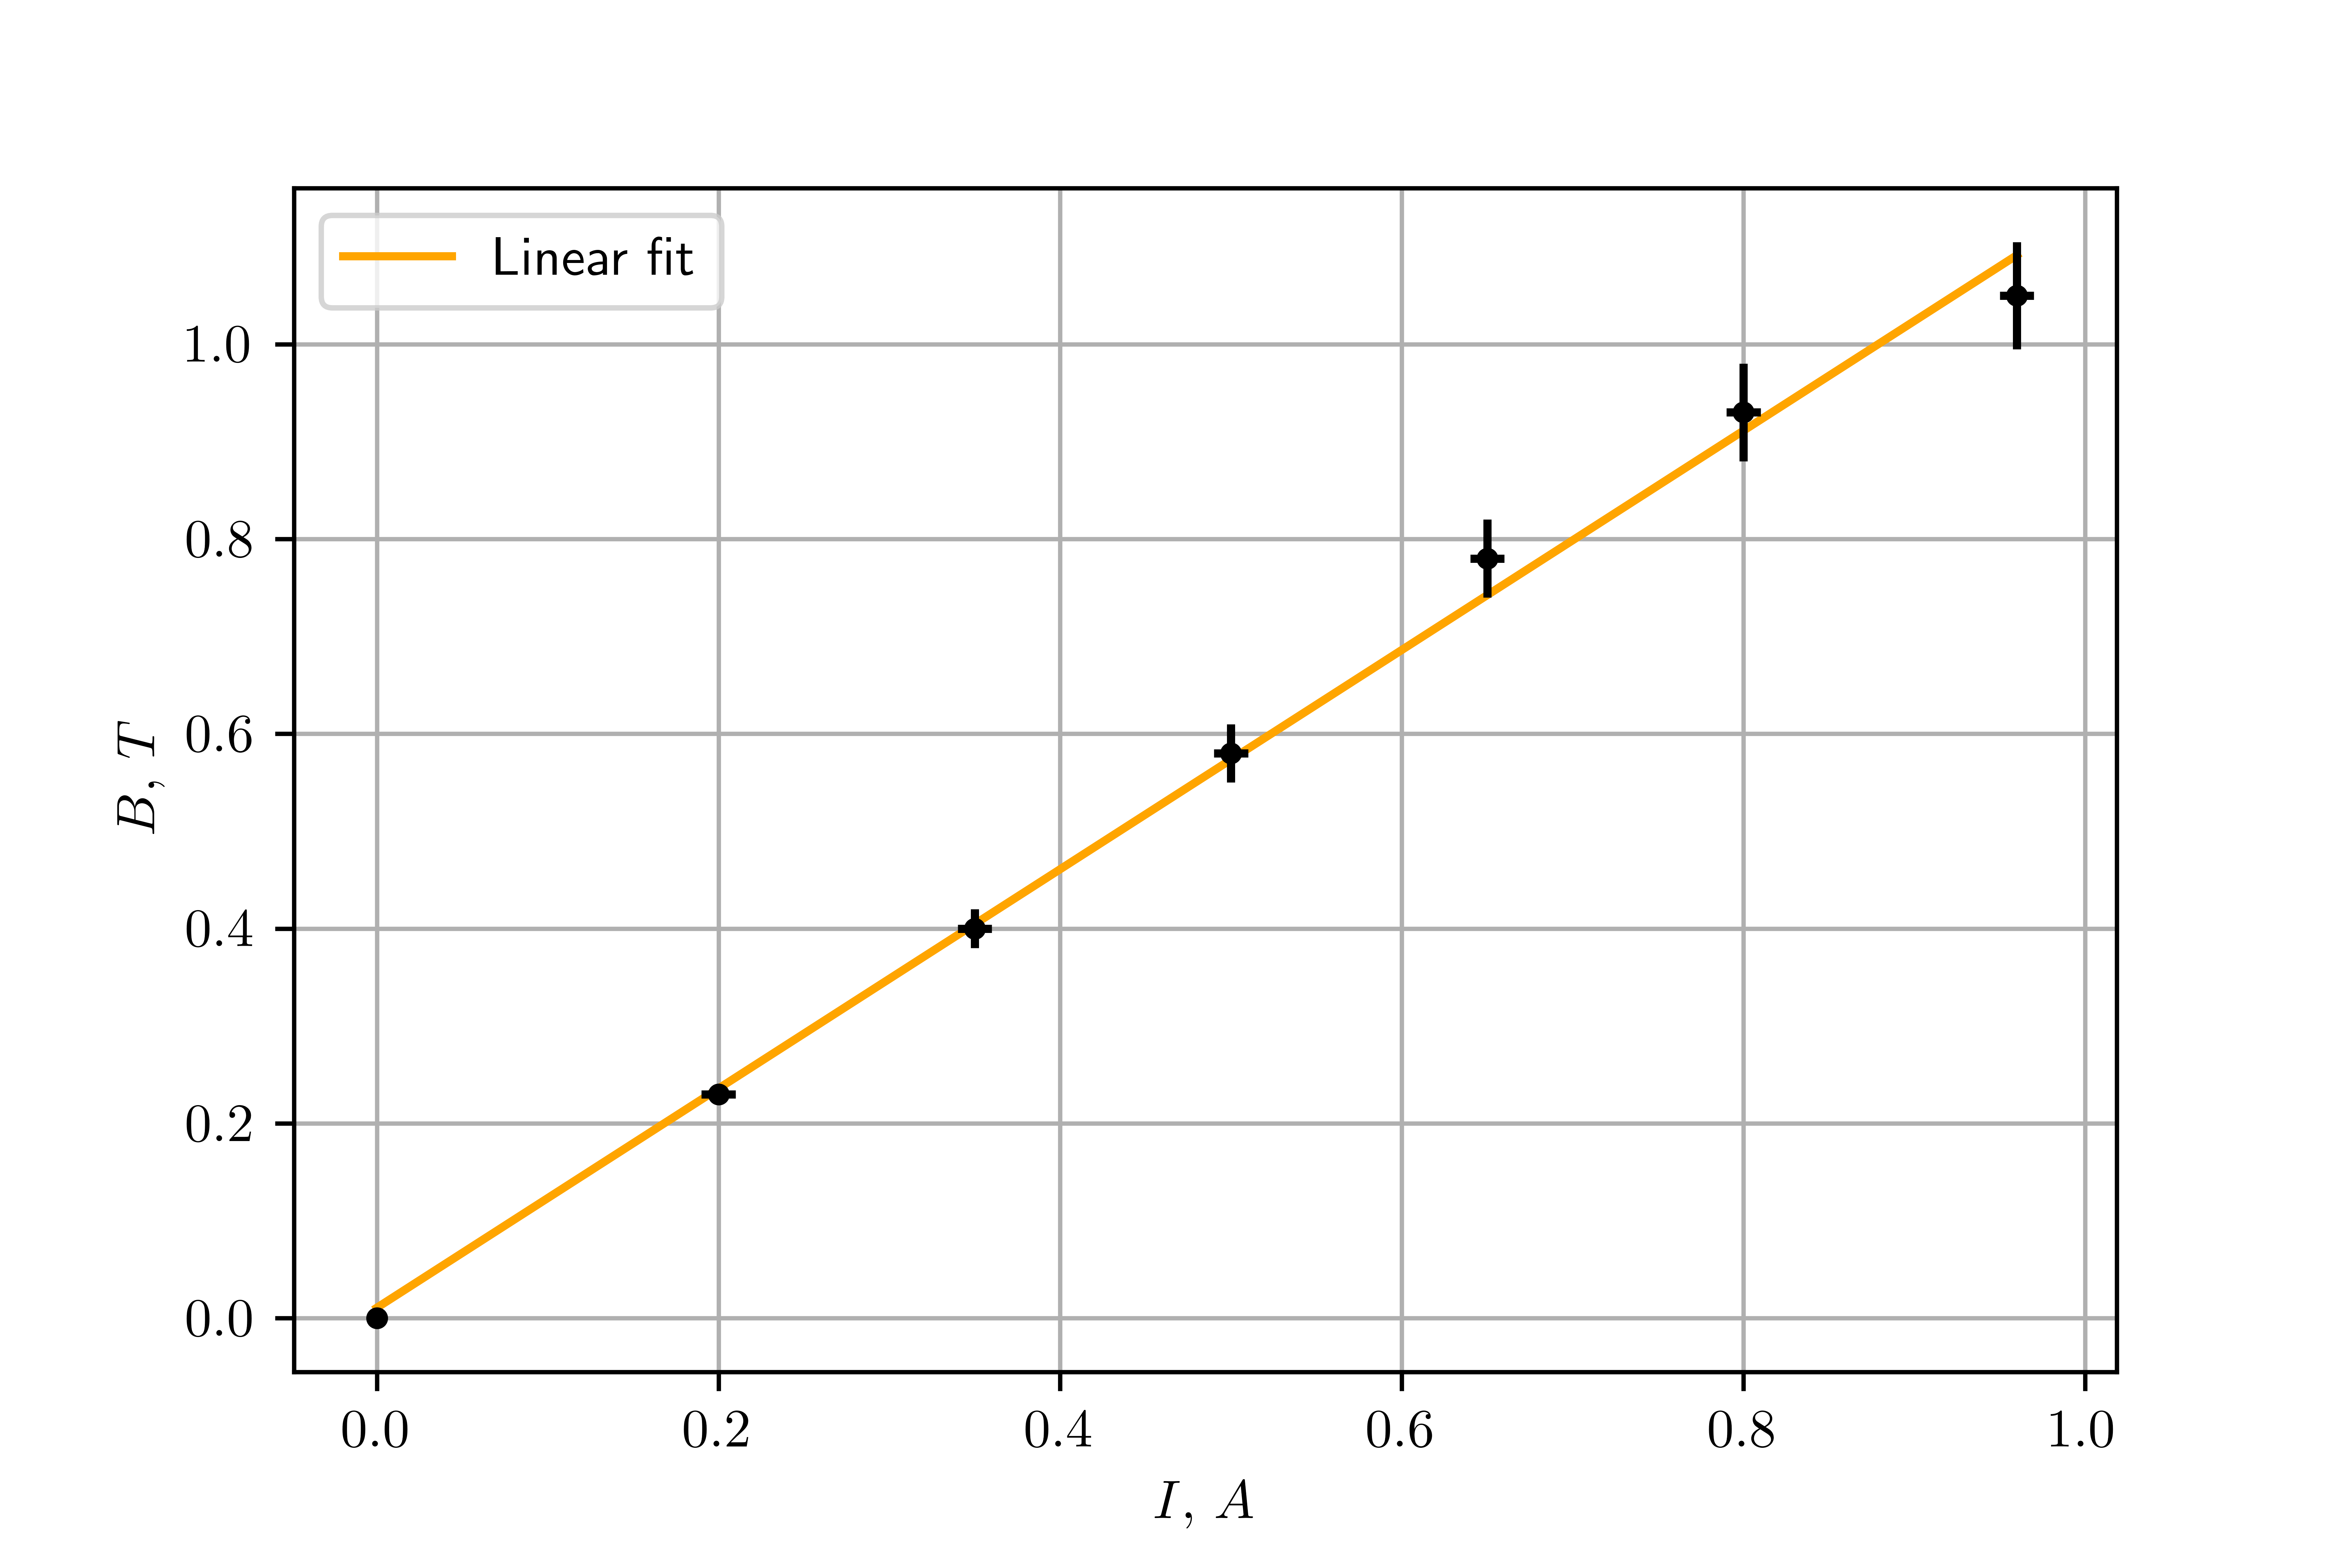
\includegraphics[width = 3cm]{PIC_4.png}
				\end{center}
				\begin{tikzpicture}
					\draw (1.5,1.5) node {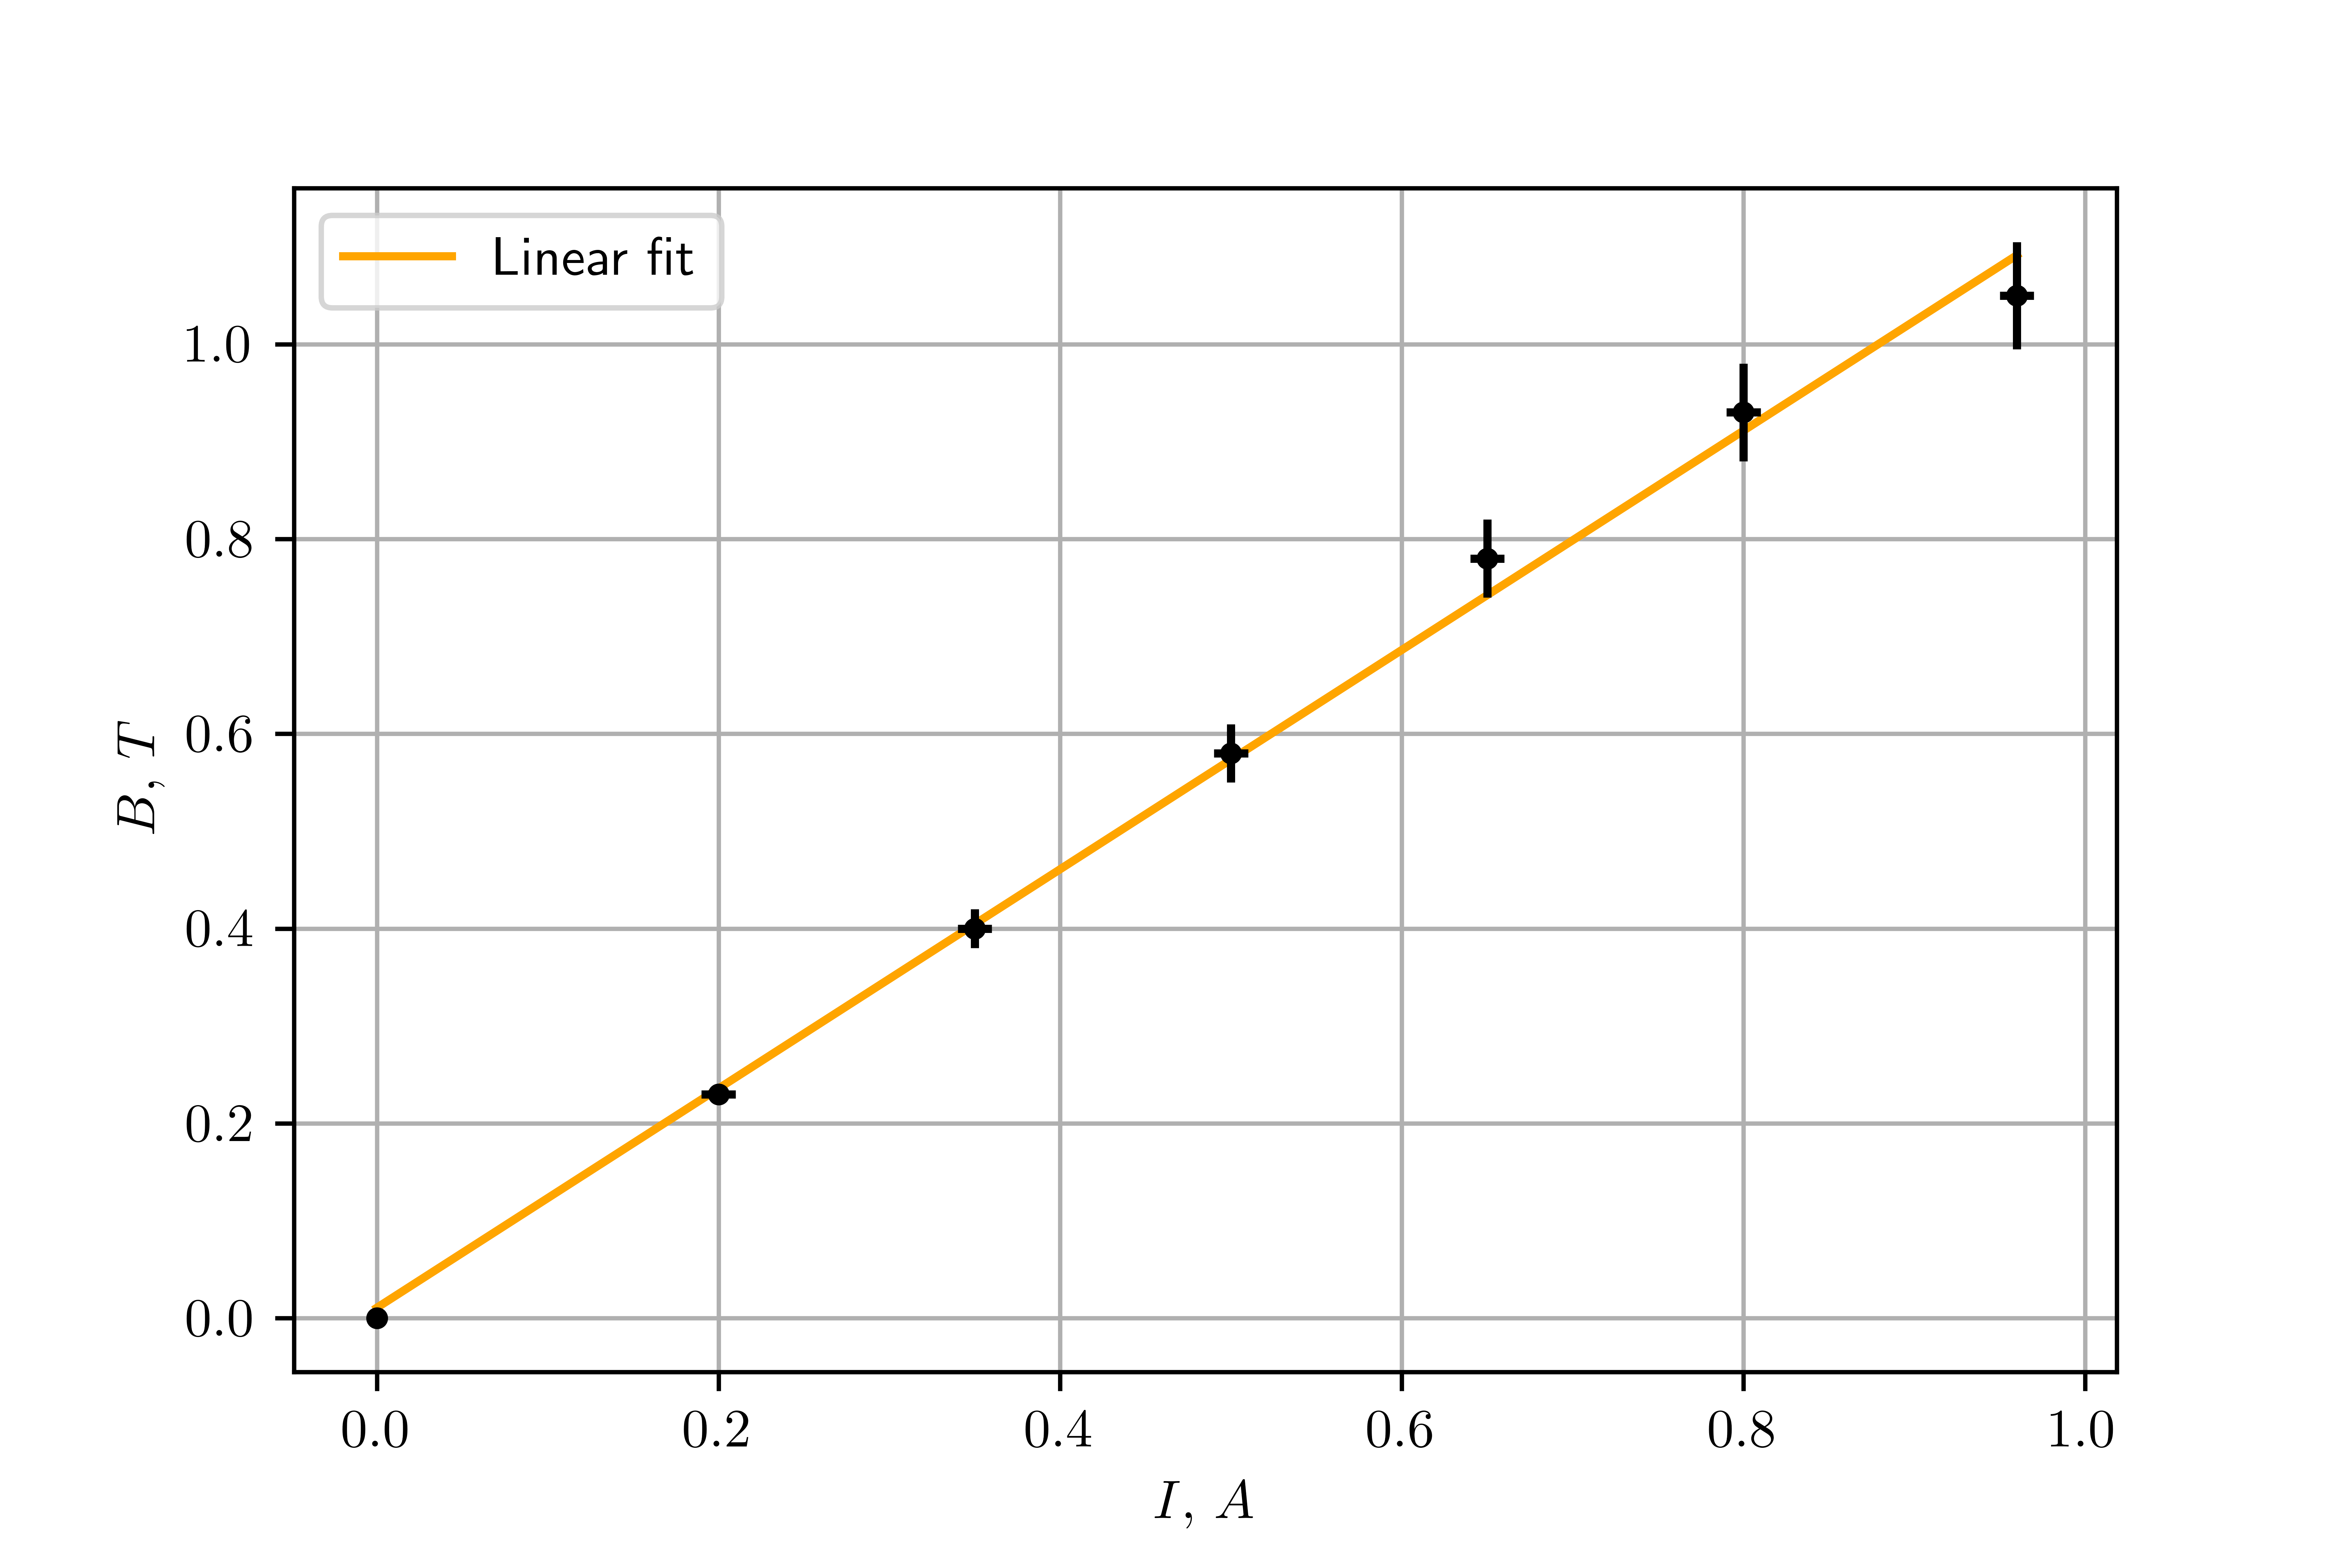
\includegraphics[width=3cm, height=3cm]{PIC_4.png}};
					\draw[black, thick] (3,0) -- (0,3);
					\draw[blue, thick, ->] (2, 1) -- (2.5, 1.5) node[above] {$\vec{E}_o$};
					\draw[blue, thick, ->] (2, 1) -- (1.5, 1.5) node[left] {$\vec{E}_e$};
					\draw[blue, thick, ->] (2, 1) -- (2.5, 0.5) node[left] {$-\vec{E}_e$};
					\draw[red, thick, ->] (2, 1) -- (2, 2);
					\draw[green, thick, ->] (2, 1) -- (3, 1);
					\draw[red, dashed] (2.5, 1.5) -- (2, 2) -- (1.5, 1.5);
					\draw[green, dashed] (2.5, 1.5) -- (3, 1) -- (2.5, 0.5);
				\end{tikzpicture}
				\stepcounter{picture}
				\textbf{Рис. 3:} Наблюдаемая интерференционная картина
			\end{minipage}
			\begin{minipage}{0.6\linewidth}
				\begin{itemize}
					\item Интерференционная картина как ожидалось -- кольца
					\item Темный мальтийский крест?
					\item Поляризация после матовой пластинки?
					\item $\Delta = 2\pi k \longrightarrow$ темное кольцо
					\item $\Delta = \pi + 2\pi k \longrightarrow$ светлое кольцо
					\item Негативный переход картины при повороте анализатора
				\end{itemize}
			\end{minipage}
		\end{figure}
	\end{frame}

	\begin{frame}
		Заметим, что из соображений закона Снеллиуса получаем радиусы темных колец:
		
		$$ r_m^2 = \frac{\lambda}{l} \frac{(n_oL)^2}{(n_o - n_e)} \cdot m $$
		
		Снимем зависимость радиуса темных колец от их номера:
		
		\embedtbl{|c|c|c|c|c|c|}{
			\hline
			$m$ & 1 & 2 & 3 & 4 & 5
			\\\hline
			$r_m$, см & 2.8 & 4.0 & 5.0 & 5.7 & 6.5
			\\\hline
		}{Зависимость $r_m(m)$}
	
		Построим график линеаризованной зависимости $r_m^2(m)$
	\end{frame}

	\begin{frame}
		\embedeps{PIC_5.eps}{0.75}{График зависимости $r_m^2(m)$}
		
		Отсюда получаем коэффициент наклона $\gamma$ и двулучепреломление:
		
		$$ \gamma = (8.53 \pm 0.18)\, \text{см}^2 \implies n_o - n_e = (0.086 \pm 0.002)$$
	\end{frame}

	\begin{frame}
		{\large Изменение характера поляризации света при наличии внешнего поля}
		
		После прохождения кристалла разность фаз между $E_\eta$ и $E_\xi$ составит:
		
		$$ \Delta = \frac{2\pi}{\lambda} \cdot2l\Delta n = \frac{4\pi}{\lambda} \frac{l}{d} AU $$
		
		 где $U = E_{ext}d$ -- напряжение на кристалле, $d = 3$ мм -- его поперечный размер, $l = 26$ мм -- длина пути луча. Поляроид пропускает горизонтальную составляющую волны. Значит, выходная напряженность складывается из проекций $E_\eta$ и $E_\xi$ на ось $\mathrm{o}X$:
		 
		 $$ E = \frac{E_0}{2} \cdot e^{i(\omega t - kl)} (e^{i\Delta/2} - e^{-i\Delta/2}) = \frac{E_0}{2} \cdot  e^{i(\omega t - kl + \pi/2)} \sin\frac{\Delta}{2} $$
	\end{frame}

	\begin{frame}
		Отсюда интенсивность выходной волны: 
		
		$$ I = I_0 \sin^2\frac{\Delta}{2} = I_0\sin^2 \left(\frac{\pi}{2}\frac{U}{U_{\lambda/2}}\right) $$
		
		Для вертикально направленного анализатора, очевидно, зависимость:
		
		$$ I = I_0 \cos^2\frac{\Delta}{2} = I_0\cos^2 \left(\frac{\pi}{2}\frac{U}{U_{\lambda/2}}\right) $$
		
		При этом вводится полуволновое напряжение $U_{\lambda/2} = \frac{\lambda}{4A}\frac{d}{l}$.
	\end{frame}

	\begin{frame}
		Соберем установку для изучения интенсивности проходящей:
		
		\embed{PPIC_2.png}{0.055}{Наблюдение интенсивности прошедшего света}
	\end{frame}

	\begin{frame}
		Как и ожидалось, при обоих положениях анализатора яркость чередуется:
		
		\begin{figure}[h]
			\begin{minipage}{0.45\linewidth}
				\embed{PIC_6.png}{0.06}{Минимум интенсивности}
			\end{minipage}
			\begin{minipage}{0.45\linewidth}
				\embed{PIC_7.png}{0.06}{Максимум интенсивности}
			\end{minipage}
		\end{figure}
		
		Запишем наблюдения напряжения на источнике:
		
		{\footnotesize \embedtbl{|c|c|c|}{
			\hline
			& $\perp$ поляризации & $\parallel$ поляризации
			\\\hline
			$U_{\lambda/2}$, ед & 27 $\pm$ 1 (max) & 26 $\pm$ 1 (min)
			\\\hline
			$2U_{\lambda/2}$, ед & 52 $\pm$ 1 (min) & 52 $\pm$ 1 (max)
			\\\hline
			$3U_{\lambda/2}$, ед & 79 $\pm$ 1 (max) & 78 $\pm$ 1 (min)
			\\\hline
			
		}{Последовательные экстремумы интенсивности}}
		
		При усреднении полуволновое напряжение:
		
			$$ U_{\lambda/2} = (390 \pm 15)\,\text{В} $$ 
	\end{frame}

	\begin{frame}
		Соберем установку для наблюдения фигур Лиссажу:

		\embed{PIC_1.png}{0.1}{Наблюдение фигур Лиссажу}
		
		Сигнал фотодатчика подается на вход $\mathrm{o}Y$ осциллографа, на ось $\mathrm{o}X$ подается переменное напряжение с источника.
	\end{frame}

	\begin{frame}
		Наблюдаем следующие фигуры Лиссажу:
		
		\begin{figure}[h]
			\begin{minipage}{0.45\linewidth}
				\embed{PIC_8.png}{0.045}{$U = U_{\lambda/2}$ при $\parallel$}
			\end{minipage}
			\begin{minipage}{0.45\linewidth}
				\embed{PIC_9.png}{0.031}{$U = 2U_{\lambda/2}$ при $\parallel$}
			\end{minipage}
			\begin{minipage}{0.45\linewidth}
				\embed{PIC_10.png}{0.045}{$U = 3U_{\lambda/2}$ при $\parallel$}
			\end{minipage}
		\end{figure}
	
		Полуволновое напряжение, определенное по фигурам Лиссажу совпадает с рассчетным.
	\end{frame}

	\begin{frame}
		{\large \textbf{Выводы:}}
		
		\begin{itemize}
			\item Исследована интерференция лазерного излучения после матовой пластинки на одноосном кристалле.
			\item Определено двулучепреломление кристалла ниобата лития на длине волны $\lambda = 630$ нм
			$$ n_o - n_e = (0.086 \pm 0.002) $$
			Значение в пределах погрешности совпадает с табличным $(n_o - n_e)_{\mathrm{ref}} = 0.084$
			\item Для данного кристалла определено полуволновое напряжение
			$$ U_{\lambda/2} = (390 \pm 15)\, \text{В} $$
			Это значение подтверждено наблюдением соответствующих фигур Лиссажу.
		\end{itemize}
	\end{frame}
\end{document}